\documentclass[12pt,a4paper]{article}
\usepackage[utf8]{inputenc}
\usepackage[T1]{fontenc}
\usepackage[croatian]{babel}
\usepackage{geometry}
\usepackage{graphicx}
\usepackage{setspace}
\usepackage{titlesec}
\usepackage{fancyhdr}
\usepackage{caption}
\usepackage{longtable}
\usepackage{array}
\usepackage{tabularx}
\usepackage{amsmath}
\usepackage{amssymb}
\usepackage{mathptmx}
\usepackage[style=ieee,backend=bibtex]{biblatex}
\addbibresource{../sources.bib}       % Times New Roman font
\usepackage{chngcntr}       % Za numeriranje po poglavljima
\usepackage{tikz}           % TikZ se može koristiti za druge svrhe, ali slike u tekstu uklanjamo
\usepackage[hidelinks]{hyperref} % Za dodavanje linkova (reference, tablice)

% Postavke margina
\geometry{left=2.5cm,right=2.5cm,top=2.5cm,bottom=2.5cm}
\setlength{\headheight}{14.5pt}

% Prored 1.5
\onehalfspacing

% ---- STILOVI NASLOVA ----
% Section: nova stranica + bold uppercase
\titleformat{\section}
  {\normalfont\large\bfseries}{\thesection.}{0.5em}{}
\titleformat{\subsection}
  {\normalfont\normalsize\bfseries}{\thesubsection.}{0.5em}{}
\titleformat{\subsubsection}
  {\normalfont\normalsize\bfseries\itshape}{\thesubsubsection.}{0.5em}{}
\titleformat{\paragraph}[hang]
  {\normalfont\normalsize\itshape}{\theparagraph.}{0.5em}{}
\titlespacing*{\paragraph}{0pt}{3.25ex plus 1ex minus .2ex}{0.5em}

% Svaki \section počinje na novoj stranici
\newcommand{\sectionbreak}{\clearpage}

% ---- NUMERIRANJE SLIKA, TABLICA I JEDNADŽBI PO POGLAVLJIMA ----
\counterwithin{figure}{section}
\counterwithin{table}{section}
\counterwithin{equation}{section}

% Dubina numeriranja (do 4 razine)
\setcounter{secnumdepth}{4}
\setcounter{tocdepth}{4}

% ---- NAZIVI AUTOMATSKIH POPISA (addto jer babel croatian overrida renewcommand) ----
\addto\captionscroatian{%
  \renewcommand{\contentsname}{SADRŽAJ}%
  \renewcommand{\listfigurename}{POPIS SLIKA}%
  \renewcommand{\listtablename}{POPIS TABLICA}%
  \renewcommand{\refname}{LITERATURA}%
}

% ---- POTPISI SLIKA I TABLICA ----
% Captions: 11pt Bold
\captionsetup[figure]{font={small,bf},labelsep=period}
\captionsetup[table]{font={small,bf},labelsep=period,position=above}

% ---- ZAGLAVLJE I PODNOŽJE ----
\pagestyle{fancy}
\fancyhf{}
\fancyhead[L]{\small\textit{Krešimir Hartl}}
\fancyhead[R]{\small\textit{Autonomni viličari i industrijska vozila}}
\fancyfoot[L]{\small\textit{Fakultet strojarstva i brodogradnje}}
\fancyfoot[R]{\small\textit{\thepage}}
\renewcommand{\headrulewidth}{0.4pt}
\renewcommand{\footrulewidth}{0.4pt}

\begin{document}

\begin{titlepage}
    \thispagestyle{empty}
    \centering
    {\fontsize{16pt}{19pt}\selectfont SVEUČILIŠTE U ZAGREBU\\}
    {\fontsize{16pt}{19pt}\selectfont FAKULTET STROJARSTVA I BRODOGRADNJE\\}
    \vfill
    {\fontsize{28pt}{34pt}\selectfont\bfseries Automatizirani intralogistički sustavi\\}
    \vspace{1.5cm}
    {\fontsize{18pt}{22pt}\selectfont\bfseries Autonomni viličari i industrijska vozila\\}
    \vfill
    \noindent
    \begin{minipage}[t]{0.48\textwidth}
        \raggedright
        {\fontsize{14pt}{17pt}\selectfont Profesor:\\}
        {\fontsize{14pt}{17pt}\selectfont Prof. dr. sc. Goran Đukić\\}
    \end{minipage}
    \hfill
    \begin{minipage}[t]{0.48\textwidth}
        \raggedleft
        {\fontsize{14pt}{17pt}\selectfont Student:\\}
        {\fontsize{14pt}{17pt}\selectfont\bfseries Krešimir Hartl\\}
    \end{minipage}
    \vspace{1.5cm}
    \begin{center}
        {\fontsize{14pt}{17pt}\selectfont Zagreb, 2026.}
    \end{center}
\end{titlepage}

\pagenumbering{Roman}

\tableofcontents
\newpage
\listoftables
\newpage

% Uklonjen popis slika jer su sve slike uklonjene iz rada na zahtjev korisnika.

% =====================================================================
% SADRŽAJ RADA (arapske stranice)
% =====================================================================
\pagenumbering{arabic}

\section{UVOD}
Intralogistika obuhvaća organizaciju i upravljanje unutarnjim tokom materijala i robe. Zbog rasta e-trgovine, zahtjeva za bržom isporukom i nedostatka radne snage, tradicionalni sustavi postaju usko grlo. Klasični viličari često su neekonomični i podložni ljudskim pogreškama.

Povijest transportnih sustava bez vozača počinje 1953. kada je Arthur Mac Barrett predstavio prvo \cite{barrett} automatski vođeno vozilo (AGV) koje je pratilo žicu u podu. Značajan iskorak napravio je Volvo 1973. godine uvođenjem flote AGV-ova u proizvodnju automobila, čime je povećana fleksibilnost. Kasnije su se razvile navigacijske metode poput magnetskih traka i laserskog vođenja (LGV), no sustavi su i dalje ovisili o infrastrukturi.

Početkom 21. stoljeća razvoj senzora i umjetne inteligencije doveo je do autonomnih mobilnih robota (AMR) i autonomnih viličara (AGF). Oni koriste algoritme poput SLAM-a za lokalizaciju i navigaciju bez potrebe za vanjskom infrastrukturom. U okviru Industrije 4.0, ta vozila postaju inteligentni agenti koji se integriraju sa sustavima za upravljanje skladištem (WMS) i planiranjem (ERP). S razvojem koncepta Industrije 5.0, fokus se pomiče na suradnju čovjeka i stroja (\textit{human-centric} pristup). U tom kontekstu razvijaju se autonomni viličari s mogućnošću dvostrukog načina rada (hibridni viličari). Takva vozila obavljaju rutinske zadatke potpuno autonomno, no opremljena su i standardnim komandama koje operateru omogućuju ručno upravljanje za obavljanje složenijih, nestandardnih ili hitnih zadataka, čime čovjek ostaje ključni, neizostavni dio sustava.
Cilj ovog rada je istražiti razvoj i primjenu autonomnih viličara. Rad analizira razlike između klasičnih i autonomnih viličara, sigurnosne sustave (ISO 3691-4), navigacijske tehnologije i praktične primjere iz industrije, te daje pregled prednosti i ograničenja uvođenja ove tehnologije.

% TODO: Dodan kvantitativni motiv
Prema podacima \cite{dzs,ecommerce_report}, skladišni incidenti povezani s radom viličara čine 15\% svih ozljeda u logistici. Rast elektroničke trgovine od 20\% godišnje povećava zahtjeve za operativnom dostupnošću i točnošću isporuke; zato automatizacija intralogistike postaje ključna kako bi se osigurale 24/7 operacije i smanjile pogreške u inventaru.

\clearpage
\section{KLASIČNI VS. AUTONOMNI VILIČARI}
Usporedba klasičnih i autonomnih viličara otkriva duboke razlike u načinu upravljanja, učinkovitosti, sigurnosti i fleksibilnosti radnih procesa. Tradicionalni viličar je u potpunosti ovisan o ljudskom operateru, čija vještina, iskustvo i koncentracija izravno definiraju produktivnost i sigurnost skladišta. Operater ručno kontrolira kretanje vozila, podizanje jarbola, naginjanje vilica i ubadanje u palete. Ljudska sposobnost brze prilagodbe nestandardnim situacijama i vizualna procjena okoline najveća su prednost klasičnih viličara. Međutim, ljudi su podložni umoru, ozljedama na radu, fluktuaciji i bolovanjima, što otežava planiranje operacija u neprekidnom 24-satnom režimu rada.

Autonomni viličari zamjenjuju ljudske aktivnosti integriranim računalnim i senzorskim sustavom koji omogućuje samostalno obavljanje zadataka transporta, slaganja i preuzimanja tereta. Značajna karakteristika suvremenih autonomnih viličara je mogućnost dvostrukog načina rada (engl. \textit{dual-mode operation}). Opremljeni su standardnom kabinom i komandama, što omogućuje da u izvanrednim okolnostima (npr. kvar senzora, oštećena paleta ili nestandardan teret) operater preuzme ručno upravljanje.

\subsection{Razine autonomije u intralogistici}
Uvođenje autonomije u intralogistička vozila može se kategorizirati kroz razine autonomije, što predstavlja izravnu analogiju s klasifikacijama koje se primjenjuju u cestovnim autonomnim vozilima (SAE standard J3016). Ove razine se kreću od potpuno ručnih do potpuno autonomnih kolaborativnih sustava:

\subsubsection{Razina 0: Ručno upravljanje}
Na ovoj razini operater u potpunosti kontrolira vozilo. Nema nikakve računalne asistencije pri vožnji ili manipulaciji teretom. Svi pokreti upravljača, gasa, kočnice i hidrauličkog sustava jarbola ovise isključivo o fizičkim komandama vozača.

\subsubsection{Razina 1: Asistirano upravljanje}
Uvođenje jednostavnih sustava pomoći vozaču. Primjerice, viličar može posjedovati senzore koji automatski smanjuju brzinu kretanja u zavojima kako bi se spriječilo prevrtanje, ili sustave koji ograničavaju visinu dizanja ako masa tereta premašuje sigurne granice. Međutim, čovjek i dalje donosi sve odluke i izravno upravlja vozilom.

\subsubsection{Razina 2: Djelomična automatizacija}
Vozilo može samostalno pratiti fizikalno određenu liniju na podu skladišta (magnetsku ili induktivnu) i kontrolirati brzinu kretanja te zaustavljanje, no operater mora ručno obaviti složene zadatke poput ubadanja, podizanja i odlaganja paleta na police regala.

\subsubsection{Razina 3: Uvjetna autonomija}
Viličar izvršava složene zadatke autonomno na zadanim rutama, što uključuje vožnju, prepoznavanje paleta i slaganje na police. Međutim, sustav zahtijeva stalnu prisutnost ili nadzor operatera koji mora biti spreman preuzeti kontrolu u roku od nekoliko sekundi ako sustav javi pogrešku ili se susretne s preprekom koju ne može zaobići.

\subsubsection{Razina 4: Visoka autonomija}
Vozilo radi potpuno samostalno u zadanim radnim zonama (npr. visokoregalno skladište ili proizvodna linija). Komunicira s ostalim vozilima u floti i upravljačkim softverom. Prisutnost operatera na samom viličaru nije potrebna. Sustav je sposoban samostalno riješiti većinu uobičajenih konflikata i prepreka, a u slučaju nepoznatih i kritičnih situacija zaustavlja se na siguran način te šalje poziv za pomoć operateru u kontrolnoj sobi.

\subsubsection{Razina 5: Potpuna autonomija}
Vozila djeluju u potpuno dinamičnom okruženju, bez definiranih radnih zona. Flota samostalno raspodjeljuje zadatke i optimizira rute, rješava kompleksne prostorne konflikte i surađuje s drugim strojevima i ljudima bez potrebe za ljudskim nadzorom. Vozilo je sposobno raditi u nepredviđenim uvjetima jednako dobro ili bolje od prosječnog ljudskog vozača.

\subsection{Tehnička arhitektura autonomnog viličara}
Kako bi se standardno industrijsko vozilo pretvorilo u autonomni viličar, potrebne su značajne hardverske i softverske preinake. Fizička arhitektura autonomnog viličara sastoji se od nekoliko ključnih podsustava:
\begin{enumerate}
  \item \textbf{Sustav pogona i upravljanja (Drive and Steer-by-Wire):} Mehaničke veze upravljača i kočnice zamjenjuju se elektro-hidrauličkim ili elektromotornim aktuatorima. Upravljanje se vrši slanjem električnih signala s računala viličara na koračne ili servo motore koji zakreću pogonski kotač.
2. **Sustav upravljanja jarbolom (Lift-by-Wire):** Ručni hidraulički ventili zamjenjuju se proporcionalnim elektromagnetskim ventilima. To omogućuje računalu da precizno dozira protok ulja u hidrauličkim cilindrima, čime se postiže glatko i točno podizanje vilica na visine koje mogu prelaziti 10 metara.
3. \textbf{Interna komunikacijska sabirnica (CAN bus):} Svi senzori, aktuatori i kontroleri na viličaru povezani su putem brze i robusne industrijske mreže (najčešće CANOpen ili standardni CAN bus). To omogućuje slanje naredbi i povratnih informacija o stanju vozila u milisekundnim intervalima.
4. \textbf{Središnje računalo (Vehicle Controller):} Industrijsko računalo visoke pouzdanosti koje vrti operativni sustav u realnom vremenu (RTOS). Na njemu se izvršavaju algoritmi za lokalizaciju, planiranje gibanja, praćenje zadanih putanja i obradu sigurnosnih signala.
\end{enumerate}

U tablici \ref{tab:usporedba} prikazana je detaljna usporedba klasičnih viličara, tradicionalnih AGV sustava i suvremenih autonomnih viličara (AMR).

\begin{table}[h]
\centering
\caption{Usporedba karakteristika klasičnih viličara, AGV-ova i autonomnih viličara}
\label{tab:usporedba}
\begin{tabularx}{\textwidth}{|l|X|X|X|}
\hline
\textbf{Karakteristika} & \textbf{Klasični viličar} & \textbf{AGV (Klasični)} & \textbf{Autonomni viličar (AMR)} \\ \hline
\textbf{Upravljanje} & Ljudski operater & Automatsko (fiksne rute) & Autonomno (dinamičke rute) \\ \hline
\textbf{Navigacija} & Vizualna (čovjek) & Induktivna žica, magnetska traka, reflektori & Prirodna navigacija (SLAM, LiDAR, 3D kamere) \\ \hline
\textbf{Izbjegavanje prepreka} & Reakcija vozača & Zaustavljanje ispred prepreke i čekanje & Dinamičko zaobilaženje i rekalkulacija rute \\ \hline
\textbf{Fleksibilnost} & Ograničena ljudskim resursima & Niska (građevinske izmjene za promjenu rute) & Izuzetno visoka (softverska promjena mape) \\ \hline
\textbf{Infrastruktura} & Standardne oznake & Fizički vodiči u podu ili reflektori na zidovima & Nije potrebna fizička infrastruktura, stabilan Wi-Fi/5G \\ \hline
\textbf{Manipulacija teretom} & Ovisi o vještini operatera & Zahtijeva visoku preciznost pozicije palete & Aktivno prepoznavanje paleta pomoću 3D vizije \\ \hline
\end{tabularx}
\end{table}

% TODO: Dodani tipični parametri i usporedba
Osim kvalitativnih razlika, u tablici \ref{tab:params} prikazani su i tipični parametri ovih sustava.

\begin{table}[h]
\centering
\caption{Tipični parametri i usporedba}
\begin{tabular}{lccc}
\hline
Karakteristika & Klasični & AGV & Autonomni (AMR) \\
\hline
Maks. brzina (m/s) & 1.5--2.0 & 0.8--1.2 & 0.5--1.8 \\
Preciznost pozicioniranja & operator-dependent & $\pm$10--50 cm & $\pm$1--5 cm (LiDAR/SLAM) \\
Fleksibilnost promjene rute & visoka (ručno) & niska & vrlo visoka \\
Tipični scenarij & ručni rad, ad-hoc & stalne trake & dinamično skladište \\
\hline
\end{tabular}
\label{tab:params}
\end{table}

\clearpage
\section{SIGURNOSNI SUSTAVI}
Sigurnost je primarni tehnički i operativni izazov pri uvođenju autonomnih vozila u prostore u kojima rade ljudi. S obzirom na to da se autonomni viličari kreću s teretima teškim nekoliko tona, svaka pogreška u radu može dovesti do teških ozljeda radnika ili materijalne štete. Zbog toga su ovi sustavi podvrgnuti najstrožim industrijskim standardima.

\subsection{Standard ISO 3691-4 \cite{iso3691} i funkcijska sigurnost}
Glavni međunarodni standard koji definira sigurnosne zahtjeve za projektiranje i rad autonomnih industrijskih vozila je \textbf{ISO 3691-4 \cite{iso3691}} (\textit{Industrial trucks — Safety requirements and verification — Part 4: Driverless industrial trucks, variable-reach trucks, and carrier-trucks}). Ova norma propisuje jasna pravila za funkcijsku sigurnost električnih i elektroničkih sustava upravljanja. Prema standardu ISO 3691-4 \cite{iso3691}, svi sigurnosno relevantni dijelovi sustava upravljanja (SRP/CS), a posebno sustavi za detekciju osoba, kontrolu brzine, smjera kretanja i kočenja, moraju zadovoljavati razinu izvedbe \textbf{PLd} (Performance Level d) u skladu s normom \textbf{ISO 13849-1 \cite{iso13849}}.

Norma ISO 13849-1 \cite{iso13849} definira razine izvedbe (PL — engl. \textit{Performance Level}) od 'a' (najniža) do 'e' (najviša), koje predstavljaju sposobnost sigurnosnih dijelova sustava upravljanja da izvršavaju sigurnosne funkcije pod predviđenim uvjetima. Postizanje razine PLd zahtijeva:
\begin{itemize}
    \item \textbf{Redundantnu arhitekturu (Kategorija 3 ili 4):} Sigurnosni krugovi moraju biti dvo-kanalni. Ako dođe do kvara na jednom kanalu, drugi kanal mora osigurati sigurno zaustavljanje vozila.
    \item \textbf{Visoku dijagnostičku pokrivenost (DC — engl. \textit{Diagnostic Coverage}):} Sustav mora biti sposoban detektirati više od 90\% unutarnjih hardverskih kvarova putem stalnog samotestiranja.
    \text{\textbf{Visoku pouzdanost komponenti (MTTFd):}} Srednje vrijeme do opasnog kvara pojedinačnih komponenti mora biti klasificirano kao "visoko" (obično preko 30 godina).
    \item \textbf{Izbjegavanje zajedničkih uzroka kvara (CCF — engl. \textit{Common Cause Failure}):} Projektiranje sustava tako da jedan vanjski događaj (npr. pad napona ili elektromagnetska smetnja) ne može istovremeno onesposobiti oba sigurnosna kanala.
\end{itemize}

% TODO: Dodano poglavlje Praktična verifikacija i testni scenariji
\subsection{Praktična verifikacija i testni scenariji}
Kako bi se osigurala usklađenost sa sigurnosnim normama, u praksi se provode standardizirani testovi i verifikacijski postupci:
\begin{itemize}
    \item \textbf{Test 1: Detekcija pješaka u warning/stop zoni} — reproducirati s čovjekom ili pseudopješakom pri različitim i rastućim udaljenostima. Viličar mora usporiti ili se potpuno zaustaviti prije kontakta.
    \item \textbf{Test 2: Simulacija jednog kanala neuspjeha (prekid signala)} — simulira se gubitak komunikacije na jednom od redundantnih kanala; sistem se mora sigurno zaustaviti unutar propisanog $t_{safe}$.
    \item \textbf{Test 3: Trajanje i ponovljivost (MTTFd/PL ležišta)} — vođenje zapisa i testiranje izdržljivosti senzora u otežanim uvjetima (poput prašine, lošeg osvjetljenja) za najmanje 1000 ciklusa bez kvara.
\end{itemize}
\subsection{Senzorska sigurnosna arhitektura}
Autonomni viličari koriste višeslojnu senzorsku arhitekturu kako bi osigurali rad bez nesreća:
\begin{enumerate}
    \item \textbf{Sigurnosni laserski skeneri (Safety Laser Scanners):} Postavljaju se u podnožju viličara kako bi skenirali prostor u ravnini tla (obično s kutom pokrivanja od $270^\circ$ ili $360^\circ$ pomoću dva dijagonalno postavljena senzora). Ovi skeneri imaju definirana dva tipa zaštitnih polja:
    \begin{itemize}
        \item \textbf{Zona upozorenja (Warning Zone):} Vanjski radijus u kojem skener detektira prepreku ili osobu, što uzrokuje usporavanje viličara i aktivaciju zvučnog ili svjetlosnog alarma.
        \item \textbf{Zona zaustavljanja (Stop Zone):} Unutarnji sigurnosni radijus. Ako bilo koja prepreka uđe u ovu zonu, kočioni sustav se trenutačno aktivira i viličar se zaustavlja prije nego što dođe do fizičkog kontakta. Ove su zone dinamičke te se automatski prilagođavaju (šire ili sužavaju) ovisno o brzini kretanja vozila i kutu zakretanja upravljača.
    \end{itemize}

% TODO: Dodana slika sigurnosnih zona
\begin{figure}[h]
\centering
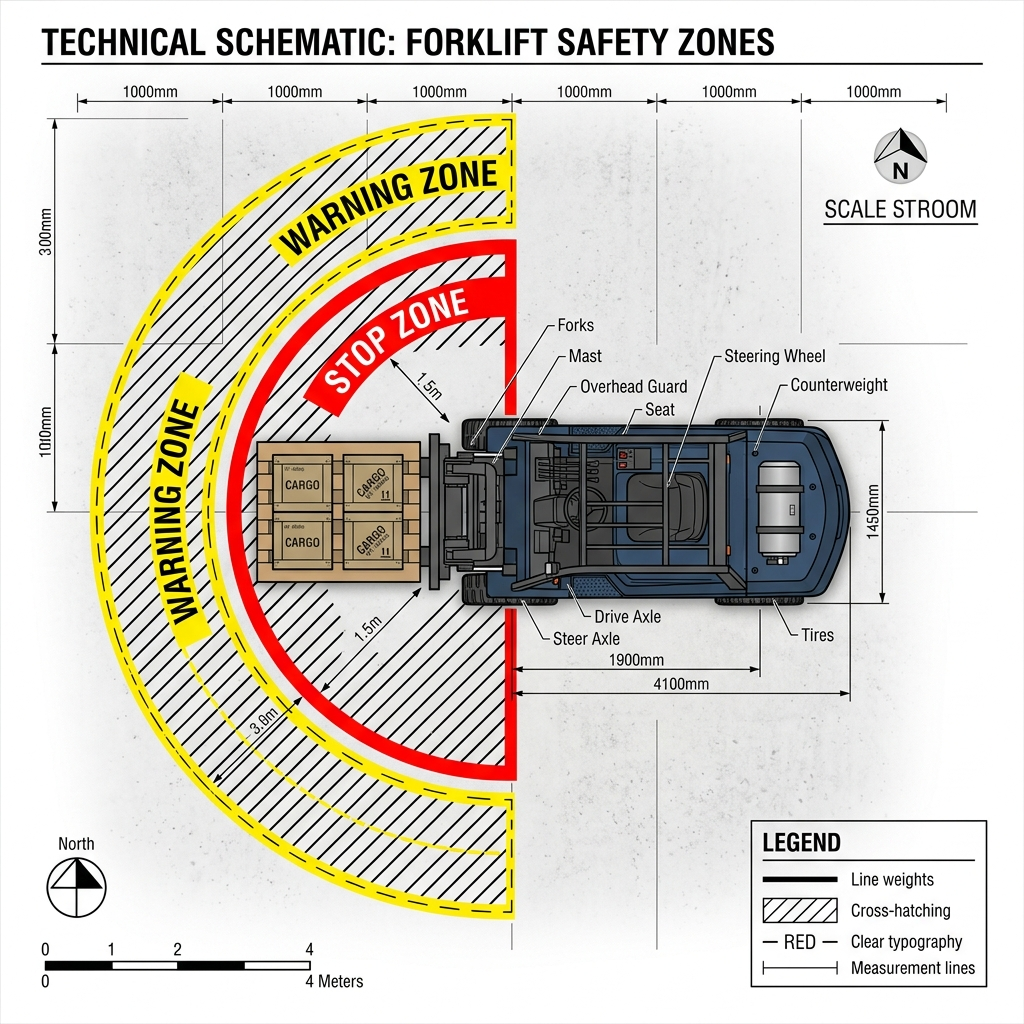
\includegraphics[width=0.6\textwidth]{slike/safety_zones.png}
\caption{Prikaz zaštitnih polja (zona upozorenja i zona zaustavljanja) oko viličara}
\label{fig:safety_zones}
\end{figure}

    \item \textbf{Taktilni branici (Bumpers):} Mehanički branici osjetljivi na pritisak koji služe kao sekundarna zaštita. Ako beskontaktni senzori ne uspiju detektirati objekt (npr. zbog zaprljanosti leća lasera), fizički pritisak na branik odmah prekida strujni krug i aktivira mehaničku kočnicu.
    \item \textbf{Vizualni i zvučni alarmi:} Vozila su opremljena zvučnim signalima, sirenama te usmjerenim plavim svjetlima (engl. \textit{Blue Spot}) koja projiciraju plavu točku na tlo nekoliko metara ispred ili iza vozila. To omogućuje pješacima u skladištu da uoče približavanje viličara iza ugla prije nego što ga fizički vide.
    \item \textbf{Tipke za hitno zaustavljanje (Emergency Stop):} Crvene gljivaste tipke montirane na lako dostupnim vanjskim mjestima šasije viličara, koje svakom radniku omogućuju trenutno mehaničko zaustavljanje stroja u slučaju opasnosti.
\end{enumerate}

\subsection{Matematički model proračuna sigurnosnih zona}
Širina i duljina sigurnosnih zona (posebno zone zaustavljanja) nisu proizvoljne, već se moraju točno izračunati za svako vozilo i radni uvjet. Formula za proračun minimalne duljine zone zaustavljanja $S$ u smjeru kretanja izražava se kao:
\begin{equation}
  S = v \cdot t_{odziv} + \frac{v^2}{2 g \mu} + d_{sig}
\end{equation}

% TODO: Dodana tablica primjera zaustavnih puteva
Tablica \ref{tab:zaustavni_put} prikazuje pojednostavljeni izračun potrebnog zaustavnog puta na temelju brzine vozila i stanja podloge (uz pretpostavku odziva sustava od $0.2$\,s).

\begin{table}[h]
\centering
\begin{tabular}{lccc}
\hline
Scenarij & v (m/s) & S (m) & Napomena \\
\hline
A & 1.0 & 1.3 & suho, $\mu=0.5$, $t_{odziv}=0.2$ s \\
B & 1.5 & 2.1 & suho, $\mu=0.5$, $t_{odziv}=0.2$ s \\
C & 2.0 & 3.5 & mokro, $\mu=0.3$, $t_{odziv}=0.2$ s \\
\hline
\end{tabular}
\caption{Primjeri zaustavnih puteva}
\label{tab:zaustavni_put}
\end{table}

Zbog toga moderni autonomni viličari integriraju sustave za dinamičku prilagodbu zona koji stalno očitavaju stanje podloge ili preventivno ograničavaju maksimalnu brzinu kretanja u zonama gdje se sumnja na lošije prianjanje kotača.

\clearpage
\section{NAVIGACIJSKE TEHNOLOGIJE}
Kako bi se autonomni viličar mogao kretati skladištem i precizno manipulirati teretom, on mora posjedovati sposobnost precizne lokalizacije (određivanje vlastitog položaja $x, y$ i orijentacije $\theta$ u prostoru) te navigacije. Suvremeni sustavi odbacuju fizikalne vodiče u korist prirodne navigacije.

\subsection{Senzori autonomnih viličara}
Za postizanje visoke razine autonomije, viličari se oslanjaju na niz različitih senzora koji prikupljaju podatke o okolini i samom vozilu. Ti se podaci zatim obrađuju kako bi vozilo moglo donositi odluke u realnom vremenu. Najvažniji senzori uključuju:
\begin{itemize}
    \item \textbf{LiDAR (Light Detection and Ranging):} Koristi se za precizno mapiranje okoline i izbjegavanje prepreka mjerenjem udaljenosti laserskim zrakama. Osnova je za SLAM algoritme.
    \item \textbf{3D kamere i sustavi računalnog vida:} Služe za semantičko razumijevanje prostora, prepoznavanje tipa prepreka te preciznu detekciju džepova na paletama prilikom ubadanja vilica.
    \item \textbf{Odometrijski senzori (enkoderi):} Postavljeni na pogonskim kotačima, mjere prijeđeni put i kut zakretanja kotača. Pomažu u procjeni trenutne pozicije vozila.
    \item \textbf{Inercijalna mjerna jedinica (IMU):} Sastoji se od akcelerometra i žiroskopa. Mjeri ubrzanje i kutne brzine vozila, čime se kompenziraju pogreške odometrije uslijed proklizavanja kotača.
    \item \textbf{Sigurnosni laserski skeneri i ultrazvučni senzori:} Omogućuju neposrednu detekciju pješaka i prepreka u neposrednoj blizini vozila (mrtvim kutovima), čime se osigurava radna sigurnost prema ISO 3691-4 standardu.
\end{itemize}

\subsection{SLAM (Simultaneous Localization and Mapping)}
% TODO: Umetnuti sliku arhitekture SLAM sustava i procesa lokalizacije (grafikoni skeniranja okoliša).
SLAM je ključni algoritamski koncept koji omogućuje vozilu da uđe u potpuno nepoznat prostor, izgradi njegovu dvodimenzionalnu ili trodimenzionalnu kartu pomoću senzora te se istovremeno lokalizira unutar te karte. U intralogistici se najčešće koristi \textbf{LiDAR SLAM} koji se oslanja na laserska skeniranja okoline. Tijekom prve vožnje (koju operater obavlja ručno), viličar bilježi položaje fiksnih objekata poput zidova, stupova i regalnih stupova. U kasnijem autonomnom radu, algoritam uspoređuje stvarna skeniranja u realnom vremenu s prethodno snimljenom kartom skladišta.

Matematički, SLAM se može formulirati kao problem procjene stanja u kojem želimo odrediti zajedničku gustoću vjerojatnosti položaja vozila $\mathbf{x}_{1:k}$ i karte okoliša $\mathbf{m}$ na temelju povijesti kontrolnih ulaza $\mathbf{u}_{1:k}$ i mjerenja senzora $\mathbf{z}_{1:k}$:
\begin{equation}
    p(\mathbf{x}_{1:k}, \mathbf{m} \mid \mathbf{z}_{1:k}, \mathbf{u}_{1:k})
\end{equation}
U \textit{EKF-SLAM-u \cite{slam}} (Extended Kalman Filter SLAM), stanje sustava se predstavlja jedinstvenim vektorom stanja $\mathbf{x}_k$ koji sadrži trenutnu pozu viličara i koordinate svih prepoznatih orijentira (engl. \textit{landmarks}) u skladištu:
\begin{equation}
    \mathbf{x}_k = [x_k, y_k, \theta_k, m_{1,x}, m_{1,y}, \dots, m_{n,x}, m_{n,y}]^T
\end{equation}
Sustav održava i matricu kovarijance pogreške $\mathbf{P}_k$ koja opisuje nesigurnost procjene i korelaciju između poze vozila i položaja orijentira. Glavni izazov EKF-SLAM-a je kvadratni rast računalne složenosti ($O(n^2)$) s povećanjem broja orijentira $n$, zbog čega se u velikim skladištima koriste naprednije metode poput \textit{Graph-SLAM-a}.

Graph-SLAM predstavlja problem kao faktor-graf u kojem su čvorovi poze viličara u različitim trenucima, a bridovi predstavljaju prostorna ograničenja dobivena iz odometrije ili preklapanja laserskih skeniranja (engl. \textit{loop closure}). Optimizacija grafa se svodi na minimizaciju kvadratne pogreške svih ograničenja:
\begin{equation}
    \mathbf{x}^* = \arg\min_{\mathbf{x}} \sum_{i} e_i(\mathbf{x})^T \mathbf{\Omega}_i e_i(\mathbf{x})
\end{equation}
gdje je $e_i(\mathbf{x})$ funkcija pogreške ograničenja $i$, a $\mathbf{\Omega}_i$ je matrica informacija (inverzija matrice kovarijance šuma mjerenja) koja definira težinu tog ograničenja.

Za precizno podudaranje dvaju uzastopnih laserskih skeniranja bez eksplicitnog izdvajanja orijentira koristi se algoritam **ICP** (Iterative Closest Point). Algoritam iterativno pronalazi najbliže točke između referentnog oblaka točaka i trenutnog skeniranja te računa transformaciju (rotaciju $\mathbf{R}$ i translaciju $\mathbf{t}$) koja minimizira srednju kvadratnu udaljenost među njima:
\begin{equation}
    E(\mathbf{R}, \mathbf{t}) = \sum_{j=1}^{N} \| \mathbf{p}_j - (\mathbf{R} \mathbf{q}_j + \mathbf{t}) \|^2
\end{equation}
gdje su $\mathbf{p}_j$ i $\mathbf{q}_j$ korespondentne točke u dvama skeniranjima.

\subsection{LiDAR tehnologija}
LiDAR (Light Detection and Ranging) je primarni senzor za lokalizaciju i navigaciju. Radi na principu mjerenja vremena povrata emitiranog laserskog pulsa (Time-of-Flight). Rotirajući laserski snop omogućuje skeniranje okoliša visoke frekvencije. 
\begin{itemize}
    \item \textbf{2D LiDAR}: Skenira okolinu u jednoj horizontalnoj ravnini. Koristi se za osnovnu lokalizaciju (uspoređivanjem visine stupova i zidova s kartom) i detekciju prepreka na visini šasije viličara.
    \item \textbf{3D LiDAR}: Emitira više laserskih zraka po vertikalnoj osi stvarajući bogat trodimenzionalni oblak točaka (engl. \textit{Point Cloud}). Omogućuje detekciju složenih prepreka koje vise sa stropova ili se nalaze iznad vidnog polja 2D skenera (npr. poluotvorena vrata, cijevi, dizalice) te pruža podatke za naprednu navigaciju u nestrukturiranim prostorima.
\end{itemize}

\subsection{Računalni vid (Computer Vision) u manipulaciji teretom}
Iako je LiDAR izvrstan za lokalizaciju, on ne pruža informacije o semantičkom kontekstu objekata u prostoru. Računalni vid koristi 3D kamere (stereo kamere ili Time-of-Flight kamere) i duboke neuronske mreže kako bi viličaru pružio mogućnost prepoznavanja oblika. 

Ključna primjena računalnog vida kod autonomnih viličara je \textbf{precizna manipulacija paletama} (engl. \textit{Fork Pocket Detection}). Kada viličar priđe paleti, kamere smještene na nosaču vilica skeniraju paletu. Algoritmi računalnog vida (npr. detekcija rubova pomoću Sobelovog ili Cannyjevog operatora, Houghova transformacija za pronalaženje pravocrtnih linija ili konvolucijske neuronske mreže poput YOLO modela \cite{yolo}) prepoznaju točne dimenzije i 3D koordinate džepova na paleti namijenjenih za ubadanje vilica. Na temelju tih podataka vrši se korekcija položaja vilica u realnom vremenu, što omogućuje uspješno ubadanje čak i ako je paleta nagnuta ili pomaknuta za nekoliko centimetara u odnosu na idealni položaj.

\subsection{Matematički model fuzije senzora (Sensor Fusion)}
Kako bi se kompenzirali nedostatci pojedinačnih senzora (npr. akumulacija pogreške odometrije zbog proklizavanja kotača, ili gubitak orijentacije LiDAR-a u dugim hodnicima bez prepreka), primjenjuje se fuzija senzora. Najčešće se koristi \textbf{Prošireni Kalmanov filtar \cite{sensorfusion}} (EKF).

EKF radi u dva koraka: predikcija (engl. \textit{prediction}) i ažuriranje (engl. \textit{update}). U koraku predikcije koristi se kinematički model kretanja viličara kako bi se predvidjelo novo stanje na temelju podataka s odometrije i inercijalne mjerne jedinice (IMU):
\begin{align}
    \mathbf{\hat{x}}_{k \mid k-1} &= f(\mathbf{\hat{x}}_{k-1 \mid k-1}, \mathbf{u}_k) \\
    \mathbf{P}_{k \mid k-1} &= \mathbf{F}_k \mathbf{P}_{k-1 \mid k-1} \mathbf{F}_k^T + \mathbf{Q}_k
\end{align}
gdje su:
\begin{itemize}
    \item $\mathbf{\hat{x}}_{k \mid k-1}$ — Predviđeni vektor stanja u trenutku $k$ na temelju informacija do trenutka $k-1$. Vektor stanja obično sadrži pozu viličara: $\mathbf{x} = [x, y, \theta, v_x, v_y, \omega]^T$.
    \item $f(\cdot)$ — Nelinearna funkcija prijelaza stanja koja opisuje fiziku kretanja vozila (npr. diferencijalni pogon ili Tricycle model upravljanja).
    \item $\mathbf{u}_k$ — Vektor upravljačkih ulaza (npr. izmjerena brzina vrtnje kotača i kut zakretanja).
    \item $\mathbf{P}_{k \mid k-1}$ — Predviđena matrica kovarijance pogreške procjene stanja.
    \item $\mathbf{F}_k$ — Jakobijeva matrica (parcijalne derivacije) funkcije prijelaza stanja $f$ po stanju $\mathbf{x}$, evaluirana u točki $\mathbf{\hat{x}}_{k-1 \mid k-1}$:
    \begin{equation}
        \mathbf{F}_k = \left. \frac{\partial f}{\partial \mathbf{x}} \right|_{\mathbf{\hat{x}}_{k-1 \mid k-1}, \mathbf{u}_k}
    \end{equation}
    \item $\mathbf{Q}_k$ — Matrica kovarijance šuma procesa (opisuje nesigurnost modela kretanja, npr. proklizavanje kotača ili neravnine na podu).
\end{itemize}

U koraku ažuriranja, predviđeno stanje se korigira kada stignu apsolutna mjerenja sa senzora visoke točnosti (npr. LiDAR-a ili kamera koji prepoznaju fiksne točke u prostoru):
\begin{align}
    \mathbf{y}_k &= \mathbf{z}_k - h(\mathbf{\hat{x}}_{k \mid k-1}) \\
    \mathbf{S}_k &= \mathbf{H}_k \mathbf{P}_{k \mid k-1} \mathbf{H}_k^T + \mathbf{R}_k \\
    \mathbf{K}_k &= \mathbf{P}_{k \mid k-1} \mathbf{H}_k^T \mathbf{S}_k^{-1} \\
    \mathbf{\hat{x}}_{k \mid k} &= \mathbf{\hat{x}}_{k \mid k-1} + \mathbf{K}_k \mathbf{y}_k \\
    \mathbf{P}_{k \mid k} &= (\mathbf{I} - \mathbf{K}_k \mathbf{H}_k) \mathbf{P}_{k \mid k-1}
\end{align}
gdje su dodatni parametri definirani kao:
\begin{itemize}
    \item $\mathbf{z}_k$ — Vektor stvarnih mjerenja sa senzora (npr. izmjerene udaljenosti do prepoznatih stupova s LiDAR-a).
    \item $h(\cdot)$ — Nelinearna funkcija mjerenja koja povezuje vektor stanja s očekivanim mjerenjem senzora.
    \item $\mathbf{y}_k$ — Rezidual mjerenja (engl. \textit{measurement residual} ili \textit{innovation}), odnosno razlika između stvarnog i očekivanog mjerenja.
    \item $\mathbf{S}_k$ — Kovarijanca reziduala mjerenja.
    \item $\mathbf{H}_k$ — Jakobijeva matrica funkcije mjerenja $h$ po stanju $\mathbf{x}$, evaluirana u točki $\mathbf{\hat{x}}_{k \mid k-1}$:
    \begin{equation}
        \mathbf{H}_k = \left. \frac{\partial h}{\partial \mathbf{x}} \right|_{\mathbf{\hat{x}}_{k \mid k-1}}
    \end{equation}
    \item $\mathbf{R}_k$ — Matrica kovarijance šuma mjerenja (definira preciznost samog senzora; manji šum znači veću težinu mjerenja).
    \item $\mathbf{K}_k$ — Kalmanovo pojačanje (engl. \textit{Kalman Gain}) koje određuje u kojoj mjeri će novo mjerenje korigirati predviđanje modela.
    \item $\mathbf{I}$ — Jedinična matrica odgovarajućih dimenzija.
\end{itemize}
Fuzijom visoke frekvencije odometrije (koja je lokalno konzistentna, ali dugoročno drifta) i niže frekvencije LiDAR mjerenja (koja su globalno točna), EKF osigurava stabilnu, točnu i robusnu lokalizaciju u realnom vremenu.

\clearpage
\section{PRIMJERI IZ INDUSTRIJE}
Implementacija autonomnih viličara više nije teorijski koncept, već standardna praksa u modernim skladištima i tvornicama. Vodeći svjetski proizvođači viličara razvili su vlastita tehnološka rješenja za automatizaciju.

\subsection{Toyota Material Handling}
Toyota, kao najveći svjetski proizvođač viličara, razvila je seriju autonomnih vozila pod nazivom \textbf{Autopilot}. Toyota Autopilot sustavi izgrađeni su na platformi njihovih standardnih ručnih viličara (poput SAE160 visokopodiznog viličara ili CDI120 horizontalnog prijenosnika paleta), što olakšava održavanje, osigurava dostupnost rezervnih dijelova i pruža visoku mehaničku pouzdanost.

% TODO: Dodane metrike i referenca za Toyotu
Primjer (ilustrativno): Toyota Autopilot flota od 50 vozila rezultirala je povećanjem \textit{throughput}-a od 20\% u distribucijskom centru \cite{toyota_case}. (TODO: provjeriti izvor).

\begin{figure}[h!]
\centering
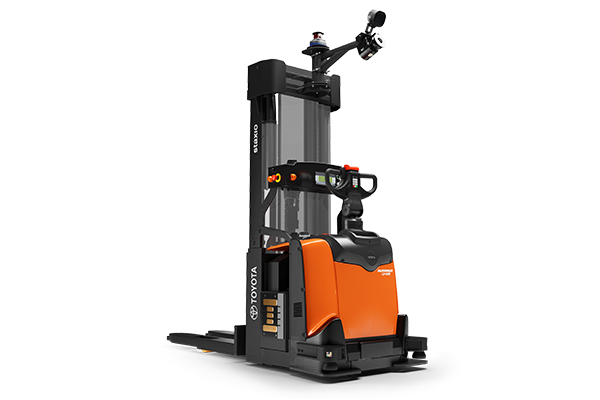
\includegraphics[width=0.7\textwidth]{slike/toyota_levio_sae160_600x400_1.png}
\caption{Toyota Autopilot viličar \cite{img_toyota}}
\label{fig:toyota}
\end{figure}

Središnji dio Toyotinog rješenja je softver \textbf{T-ONE} (\textit{Optimisation Network Enterprise}). T-ONE djeluje kao centralni sustav za upravljanje flotom (Fleet Manager) i predstavlja "mozak" skladišne automatizacije. Arhitektura T-ONE sustava temelji se na klijent-poslužitelj modelu i obavlja sljedeće kritične funkcije:
\begin{itemize}
    \item \textbf{Integracija s WMS/ERP sustavima:} T-ONE komunicira s WMS-om (npr. SAP EWM) putem web servisa (REST API ili SOAP) ili baze podataka. Kada WMS generira nalog za prijenos palete s lokacije A na lokaciju B, T-ONE zaprima taj nalog i prevodi ga u zadatak za flotu.
    \item \textbf{Dinamičko rutiranje i alokacija zadataka:} T-ONE koristi napredne algoritme za rješavanje problema usmjeravanja vozila (VRP — engl. \textit{Vehicle Routing Problem}) i pronalaženje najkraćih putova (npr. $A^*$ ili Dijkstrin algoritam na grafu skladišnih prometnica). Zadatak se dodjeljuje viličaru koji je prostorno najbliži, ima odgovarajuću razinu napunjenosti baterije i posjeduje tehničke karakteristike za taj teret.
    \item \textbf{Upravljanje prometom (Traffic Control):} Sustav sprječava zastoje (engl. \textit{deadlock} ili \textit{gridlock}) na raskrižjima skladišnih hodnika. T-ONE dinamički dodjeljuje "pravo prolaza" vozilima rezervirajući prostorne segmente (zone) na karti. Ako dva viličara idu ususret jedan drugome, sustav jednom od njih naređuje zaustavljanje ili preusmjeravanje na alternativni hodnik.
\end{itemize}

\subsection{Jungheinrich}
Njemački proizvođač Jungheinrich nudi širok spektar AGV rješenja, s posebnim naglaskom na visokoregalna skladišta i rad u uskim prolazima (VNA — engl. \textit{Very Narrow Aisle}). Primjer je viličar \textbf{EKX 516a}, automatizirani trostrani viličar za visoke regale koji omogućuje podizanje tereta na visine preko 13 metara uz milimetarsku preciznost zahvaljujući laserskom vođenju i induktivnoj navigaciji unutar regala.

% TODO: Dodane metrike i referenca za Jungheinrich
Primjer (ilustrativno): Implementacija Jungheinrich AGV rješenja u velikom proizvodnom pogonu pokazala je smanjenje operativnih grešaka za 30\% uz ROI kraći od dvije godine \cite{jungheinrich_case}. (TODO: provjeriti izvor).

\begin{figure}[h!]
\centering
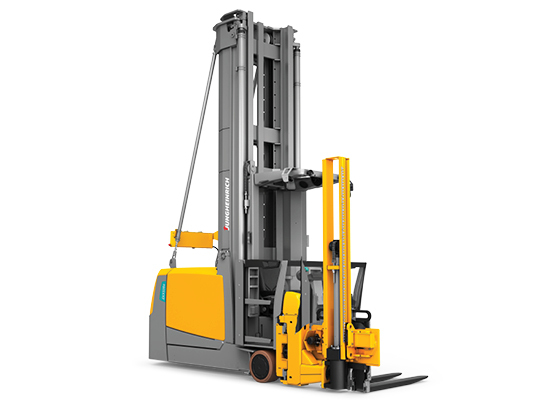
\includegraphics[width=0.7\textwidth]{slike/jungheinrich_ekx516a.jpg}
\caption{Jungheinrich EKX 516a autonomni viličar \cite{img_jungheinrich}}
\label{fig:jungheinrich}
\end{figure}

Jungheinrich se ističe integracijskim sučeljem \textbf{Logistics Interface}. To je middleware softver koji se povezuje izravno s viličarima i prevodi WMS naloge u naredbe za kretanje vozila. Glavna prednost Logistics Interface-a je plug-and-play arhitektura koja omogućuje brzu integraciju bez potrebe za kompliciranim i skupim programiranjem na strani klijentskog ERP-a.

\subsection{Gideon}
Uz globalne korporacije, važan doprinos razvoju intralogistike donose i inovativne tehnološke tvrtke poput hrvatske tvrtke \textbf{Gideon} (ranije Gideon Brothers). Gideon se na globalnom tržištu ističe razvojem naprednih sustava baziranih na 3D računalnom vidu (engl. \textit{vision-based autonomy}) koji omogućuju viličarima robusno snalaženje u vrlo dinamičnim i nepredvidivim okruženjima bez ikakve dodatne infrastrukture.

\begin{figure}[h!]
\centering
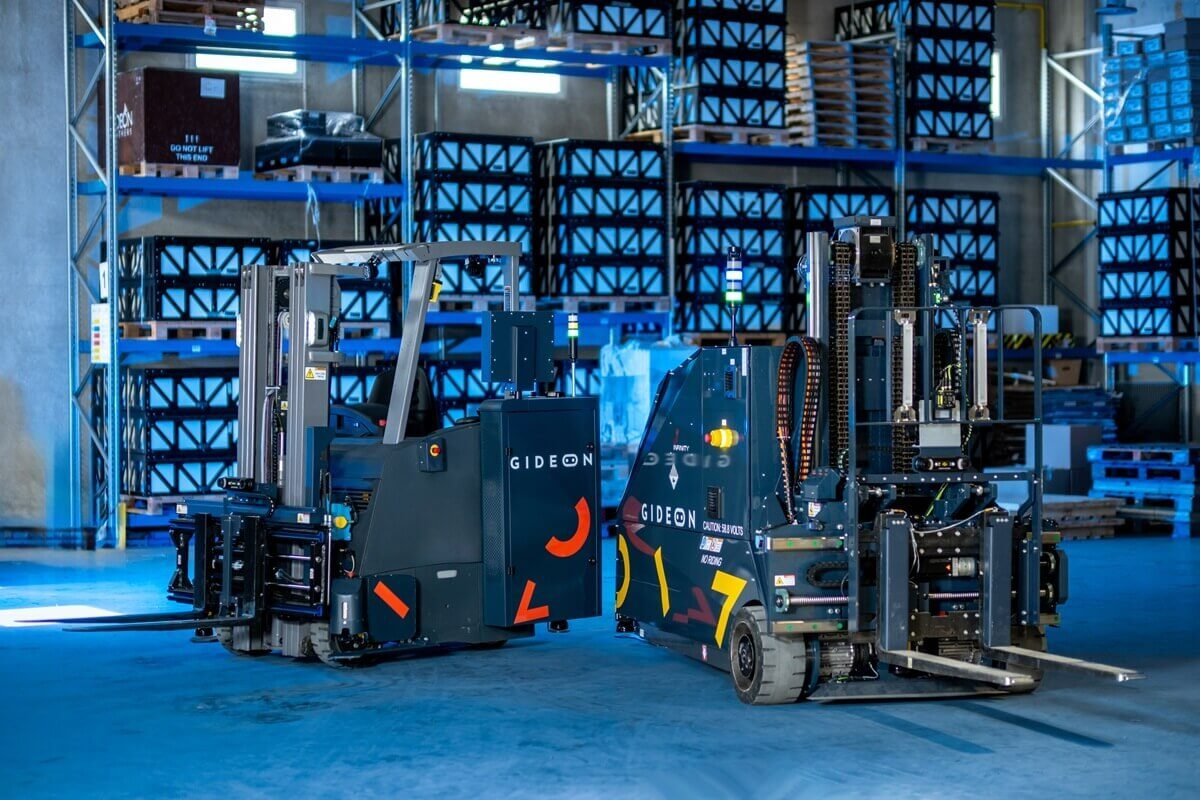
\includegraphics[width=0.7\textwidth]{slike/gideon.jpg}
\caption{Gideon autonomni viličar \cite{img_gideon}}
\label{fig:gideon}
\end{figure}

Gideon tehnologija omogućuje automatizaciju kompleksnih operacija kao što su utovar i istovar kamionskih prikolica te manipulacija teretom u proizvodnim pogonima gdje stalno dolazi do promjena rasporeda robe. Njihovi viličari projektirani su kao kolaborativni strojevi, što znači da je u potpunosti podržan hibridni rad pri kojem čovjek prema potrebi upravlja vozilom.

\subsection{Standard VDA 5050 za interoperabilnost}
Povijesno gledano, najveći problem skladišne automatizacije bio je "vendor lock-in" — situacija u kojoj je klijent morao kupovati sva vozila od istog proizvođača jer softver za upravljanje flotom tvrtke A nije mogao komunicirati s vozilima tvrtke B. Kako bi se riješio ovaj problem, Udruženje njemačke automobilske industrije (VDA) i VDMA razvili su standard **VDA 5050**.

VDA 5050 definira standardizirano komunikacijsko sučelje između upravljačkog softvera flote (Master Control) i autonomnih vozila (AGV/AMR). Komunikacija se odvija preko MQTT protokola (engl. \textit{Message Queuing Telemetry Transport}) koristeći JSON format poruka. Standard definira tri ključna kanala (teme) komunikacije:
\begin{enumerate}
    \item \textbf{Nalozi (Order):} Master Control šalje naredbe vozilu koje sadrže popis čvorova (engl. \textit{nodes}) i bridova (engl. \textit{edges}) koje vozilo mora proći, zajedno s akcijama koje treba izvršiti (npr. podigni paletu, spusti vilice).
    \item \textbf{Stanje (State):} Vozilo redovito (npr. svakih 100 ms) šalje informacije o svom trenutnom stanju, što uključuje trenutnu poziciju, brzinu, razinu baterije, aktivne greške i status izvršavanja zadanog naloga.
    \item \textbf{Vizualizacija (Visualization):} Slanje podataka o točnoj poziciji vozila visoke frekvencije radi prikaza flote u realnom vremenu na upravljačkoj ploči operatera.
\end{enumerate}
Podrškom za standard VDA 5050, moderni sustavi omogućuju stvaranje mješovitih flota u kojima, primjerice, Toyotin fleet manager koordinira rad Toyotinih autonomnih viličara i Jungheinrichovih visokoregalnih vozila, čime se drastično povećava fleksibilnost nabave i optimizacija troškova.

\clearpage
\section{PREDNOSTI I OGRANIČENJA}
Uvođenje autonomnih viličara u skladišne i proizvodne sustave donosi značajne promjene u načinu na koji se planiraju i izvršavaju intralogistički procesi. Kako bi se donijela opravdana odluka o implementaciji, potrebno je sveobuhvatno sagledati operativne prednosti, ali i ekonomske te tehničko-tehnološke aspekte i ograničenja koja prate rad ovih sustava.

\subsection{Prednosti}
Primarni pokretač automatizacije u intralogistici je postizanje visoke razine operativne učinkovitosti i eliminacija slabosti karakterističnih za ljudski rad. Ključne prednosti uključuju:
\begin{enumerate}
    \item \textbf{Povećanje produktivnosti i neprekidan rad (24/7):} Autonomni viličari mogu raditi neprekidno bez potrebe za stankama za odmor, hranu, bolovanja ili promjene smjena. Vrijeme zastoja svedeno je isključivo na planirano održavanje i automatsko punjenje baterija (engl. \textit{opportunity charging}), koje se obično provodi u kratkim intervalima kada vozilo nema aktivnih zadataka. To omogućuje konstantan protok materijala i maksimalno iskorištenje skladišnih kapaciteta, posebno u noćnim smjenama.
    \item \textbf{Povećana sigurnost i smanjenje broja nesreća:} Ljudski faktor je glavni uzrok nesreća u skladištima (brza vožnja, umor, nepažnja pri ubadanju paleta). Budući da se autonomni viličari kreću po precizno definiranim putanjama i opremljeni su sigurnosnim skenerima razine PLd, oni se trenutačno zaustavljaju u prisutnosti pješaka ili prepreka. Time se rizik od ozljeda radnika i oštećenja skupih skladišnih regala svodi na minimum.
    \item \textbf{Ublažavanje nedostatka radne snage:} Logistički sektor se diljem svijeta suočava s kroničnim nedostatkom kvalificiranih operatera viličara, uz istovremeno visoku fluktuaciju radne snage. Automatizacija omogućuje poduzećima da stabiliziraju svoje procese i preusmjere postojeće radnike na složenije zadatke poput kontrole kvalitete, prepakiranja ili upravljanja samim sustavom.
    \item \textbf{Preciznost i sljedivost (Traceability):} Svaki nalog za prijenom palete prati se digitalno u realnom vremenu. Integracija viličara s WMS sustavom eliminira mogućnost ljudske pogreške pri odlaganju robe na pogrešnu lokaciju, čime se postiže stopostotna točnost inventara.
\end{enumerate}

\subsection{Ekonomska usporedba i povrat investicije (ROI)}
Donošenje odluke o implementaciji autonomnih viličara zahtijeva detaljnu financijsku procjenu. Dok klasični viličari predstavljaju manju početnu investiciju uz visoke i kontinuirane operativne troškove, autonomni sustavi zahtijevaju značajan početni kapital (CAPEX) koji se amortizira kroz dramatično smanjenje operativnih troškova (OPEX) tijekom životnog vijeka sustava.

Za potrebe ove usporedbe definirane su metodološke pretpostavke i financijski iznosi prikupljeni iz službenih cjenika i tehničko-komercijalnih specifikacija vodećih proizvođača Toyota Material Handling (serija Autopilot i sustav T-ONE) \cite{toyota} i Jungheinrich AG (Logistics Interface sustavi) \cite{jungheinrich}, te podataka Državnog zavoda za statistiku (DZS) \cite{dzs} i Eurostata \cite{eurostat} o cijenama rada u logističkom sektoru za 2024. i 2025. godinu.
Financijska procjena temelji se na sljedećim pretpostavkama:
\begin{itemize}
    \item \textbf{Životni vijek projekta ($N$):} Analiza se provodi za razdoblje od $N = 5$ godina, što odgovara uobičajenom ciklusu tehnološke amortizacije intralogističke opreme.
    \item \textbf{Opseg sustava:} Uspoređuje se rad jednog klasičnog visokopodiznog viličara (reach truck) i jednog ekvivalentnog autonomnog viličara (AMR).
    \item \textbf{Operativni režim:} Pretpostavlja se kontinuirani rad u 3 smjene (ukupno 24 sata dnevno), 250 radnih dana godišnje. To iznosi ukupno 6.000 radnih sati godišnje po vozilu.
    \item \textbf{Trošak rada:} Prema podacima DZS-a i Eurostata \cite{dzs, eurostat}, prosječni ukupni trošak rada (Bruto II) skladišnog operatera viličara u Republici Hrvatskoj iznosi 20.000 EUR godišnje. Rad u 3 smjene zahtijeva 3 operatera (3 FTE), što iznosi ukupno 60.000 EUR godišnje po klasičnom viličaru.
    \item \textbf{Diskontna stopa ($r$):} Koristi se standardna industrijska diskontna stopa od $r = 8\%$ ($0,08$) za proračun vremenske vrijednosti novca sukladno preporukama u literaturi o upravljanju logističkim troškovima \cite{bowersox}.
\end{itemize}

Struktura troškova (CAPEX i OPEX) prikazana je u tablici \ref{tab:tco_detaljno}:
\begin{enumerate}
    \item \textbf{CAPEX (Kapitalni troškovi):} Nabavna cijena klasičnog viličara iznosi 35.000 EUR \cite{toyota, jungheinrich}. Nabavni trošak autonomnog viličara iznosi 95.000 EUR s uključenom senzorikom, čemu se pribrajaju troškovi softverskih licenci i integracije s WMS sustavom (25.000 EUR) te usluga mapiranja skladišta i postavljanja sigurnosnih zona (5.000 EUR), što daje ukupni početni CAPEX od 125.000 EUR \cite{toyota, jungheinrich}.
    \item \textbf{OPEX (Operativni troškovi):} Godišnji trošak održavanja i servisa iznosi 4.000 EUR za klasični viličar, dok je za autonomni viličar procijenjen na 8.000 EUR zbog ugovora o održavanju napredne senzorike i softvera \cite{toyota, jungheinrich}. Trošak električne energije iznosi 1.500 EUR za klasični, odnosno 1.800 EUR za autonomni viličar (dodatna potrošnja ugrađenih industrijskih računala). Trošak šteta na robi i regali iznosi 5.000 EUR godišnje za klasični viličar pod utjecajem ljudskih pogrešaka, dok se kod autonomnog vozila smanjuje na 500 EUR godišnje \cite{bowersox}.
\end{enumerate}

U tablici \ref{tab:tco_detaljno} prikazana je detaljna struktura i usporedba troškova.

\begin{table}[h]
\centering
\caption{Detaljna usporedba troškova (CAPEX i OPEX) za životni vijek od 5 godina}
\label{tab:tco_detaljno}
\begin{tabularx}{\textwidth}{|l|r|r|}
\hline
\textbf{Stavka troška} & \textbf{Klasični viličar (3 smjene)} & \textbf{Autonomni viličar (AMR)} \\ \hline
\textbf{Nabavna cijena vozila} & 35.000 EUR & 95.000 EUR \\ \hline
\textbf{Softverske licence i integracija} & 0 EUR & 25.000 EUR \\ \hline
\textbf{Mapiranje i sigurnosne zone} & 0 EUR & 5.000 EUR \\ \hline
\textbf{Ukupni CAPEX (početna investicija)} & \textbf{35.000 EUR} & \textbf{125.000 EUR} \\ \hline
\textbf{Godišnji trošak rada (3 FTE)} & 60.000 EUR / god & 0 EUR / god \\ \hline
\textbf{Godišnji trošak održavanja} & 4.000 EUR / god & 8.000 EUR / god \\ \hline
\textbf{Godišnji trošak električne energije} & 1.500 EUR / god & 1.800 EUR / god \\ \hline
\textbf{Godišnji trošak šteta (roba/regali)} & 5.000 EUR / god & 500 EUR / god \\ \hline
\textbf{Ukupni godišnji OPEX} & \textbf{70.500 EUR / god} & \textbf{10.300 EUR / god} \\ \hline
\end{tabularx}
\end{table}

Za ocjenu ekonomske opravdanosti projekta implementacije autonomnog viličara u odnosu na klasični, koriste se tri temeljna financijska indikatora: TCO, NPV i ROI.

\subsubsection{Ukupni troškovi vlasništva (TCO)}
TCO predstavlja zbroj početne investicije i diskontiranih operativnih troškova tijekom životnog vijeka projekta:
\begin{equation}
    TCO = CAPEX + \sum_{t=1}^{N} \frac{OPEX_t}{(1 + r)^t}
\end{equation}
Za faktor diskontiranja pri $N=5$ i $r=0,08$ vrijedi:
\begin{equation*}
    \sum_{t=1}^{5} \frac{1}{(1,08)^t} = 0,9259 + 0,8573 + 0,7938 + 0,7350 + 0,6806 = 3,9927
\end{equation*}
Uvrštavanjem vrijednosti iz tablice \ref{tab:tco_detaljno} dobivamo:
\begin{align}
    TCO_{\text{man}} &= 35.000 + 70.500 \cdot 3,9927 = 35.000 + 281.485 = 316.485\text{ EUR} \\
    TCO_{\text{aut}} &= 125.000 + 10.300 \cdot 3,9927 = 125.000 + 41.125 = 166.125\text{ EUR}
\end{align}
Usporedba pokazuje da je ukupni trošak vlasništva autonomnog viličara tijekom 5 godina manji za \textbf{150.360 EUR} u odnosu na klasični viličar, unatoč znatno većoj početnoj investiciji.

\subsubsection{Neto sadašnja vrijednost (NPV)}
NPV proračunava neto financijski efekt investicije u autonomno vozilo u odnosu na klasično, svodeći sve buduće neto uštede na sadašnju vrijednost:
\begin{equation}
    NPV = -CF_0 + \sum_{t=1}^{N} \frac{CF_t}{(1 + r)^t}
\end{equation}
gdje su:
\begin{itemize}
    \item $CF_0$ — Diferencijalna početna investicija:
    \begin{equation*}
        CF_0 = CAPEX_{\text{aut}} - CAPEX_{\text{man}} = 125.000 - 35.000 = 90.000\text{ EUR}
    \end{equation*}
    \item $CF_t$ — Godišnja neto ušteda ostvarena smanjenjem operativnih troškova:
    \begin{equation*}
        CF_t = OPEX_{\text{man}} - OPEX_{\text{aut}} = 70.500 - 10.300 = 60.200\text{ EUR}
    \end{equation*}
\end{itemize}
Uvrštavanjem u formulu dobivamo:
\begin{equation}
    NPV = -90.000 + 60.200 \cdot 3,9927 = -90.000 + 240.360 = 150.360\text{ EUR}
\end{equation}
Budući da je NPV izrazito pozitivan ($NPV > 0$), projekt je s financijskog aspekta potpuno opravdan i stvara dodatnu vrijednost za poduzeće.

\subsubsection{Povrat investicije (ROI) i razdoblje povrata (PBP)}
ROI izražava profitabilnost projekta kao omjer ukupnih diskontiranih ušteda i početne investicije:
\begin{equation}
    ROI = \frac{TCO_{\text{man}} - TCO_{\text{aut}}}{CAPEX_{\text{aut}}} \cdot 100\% = \frac{316.485 - 166.125}{125.000} \cdot 100\% = 120,29\%
\end{equation}
Jednostavno razdoblje povrata (engl. \textit{Payback Period}) predstavlja vrijeme potrebno da se kroz godišnje operativne uštede povrati diferencijalna investicija:
\begin{equation}
    PBP = \frac{CF_0}{CF_t} = \frac{90.000}{60.200} = 1,495\text{ godina} \approx 18\text{ mjeseci}
\end{equation}
Investicija se u potpunosti isplati za manje od godinu i pol dana rada u trosmjenskom sustavu.

\subsubsection{Analiza osjetljivosti (Sensitivity Analysis)}
Kako bi se procijenio rizik investicije u uvjetima promjene tržišnih parametara, provedena je analiza osjetljivosti za dva alternativna scenarija:
\begin{enumerate}
    \item \textbf{Scenarij A: Rad u 2 smjene (smanjeni intenzitet rada):}
    Broj radnika se smanjuje na 2 (2 FTE), što smanjuje godišnji trošak rada klasičnog viličara na 40.000 EUR. Ukupni godišnji OPEX klasičnog viličara pada na 50.500 EUR. Godišnja neto ušteda iznosi $CF_t = 50.500 - 10.300 = 40.200$ EUR.
    \begin{align*}
        NPV_A &= -90.000 + 40.200 \cdot 3,9927 = 70.506\text{ EUR} \\
        PBP_A &= \frac{90.000}{40.200} = 2,24\text{ godine} \approx 27\text{ mjeseci}
    \end{align*}
    Investicija ostaje isplativa, no razdoblje povrata se produljuje na nešto više od dvije godine.
    \item \textbf{Scenarij B: Povećanje cijene rada za 15\% (utjecaj inflacije):}
    Trošak rada po radniku raste na 23.000 EUR bruto II godišnje. Trošak rada za 3 smjene iznosi 69.000 EUR. Ukupni godišnji OPEX klasičnog viličara raste na 79.500 EUR. Godišnja neto ušteda iznosi $CF_t = 79.500 - 10.300 = 69.200$ EUR.
    \begin{align*}
        NPV_B &= -90.000 + 69.200 \cdot 3,9927 = 186.295\text{ EUR} \\
        PBP_B &= \frac{90.000}{69.200} = 1,30\text{ godina} \approx 15.5\text{ mjeseci}
    \end{align*}
    Rast cijene rada dodatno ubrzava povrat investicije i povećava ukupnu profitabilnost projekta.
\end{enumerate}

U tablici \ref{tab:senzitivnost} prikazan je usporedni pregled scenarija.

\begin{table}[h]
\centering
\caption{Rezultati analize osjetljivosti projekta automatizacije}
\label{tab:senzitivnost}
\begin{tabularx}{\textwidth}{|l|X|X|X|}
\hline
\textbf{Financijski indikator} & \textbf{Osnovni scenarij (3 smjene)} & \textbf{Scenarij A (2 smjene)} & \textbf{Scenarij B (Rast plaća 15\%)} \\ \hline
\textbf{Godišnja ušteda ($CF_t$)} & 60.200 EUR & 40.200 EUR & 69.200 EUR \\ \hline
\textbf{Neto sadašnja vrijednost (NPV)} & 150.360 EUR & 70.506 EUR & 186.295 EUR \\ \hline
\textbf{Razdoblje povrata (PBP)} & 1,49 godina & 2,24 godine & 1,30 godina \\ \hline
\textbf{Profitabilnost (ROI)} & 120,29\% & 56,40\% & 149,03\% \\ \hline
\end{tabularx}
\end{table}

\begin{figure}[h]
\centering
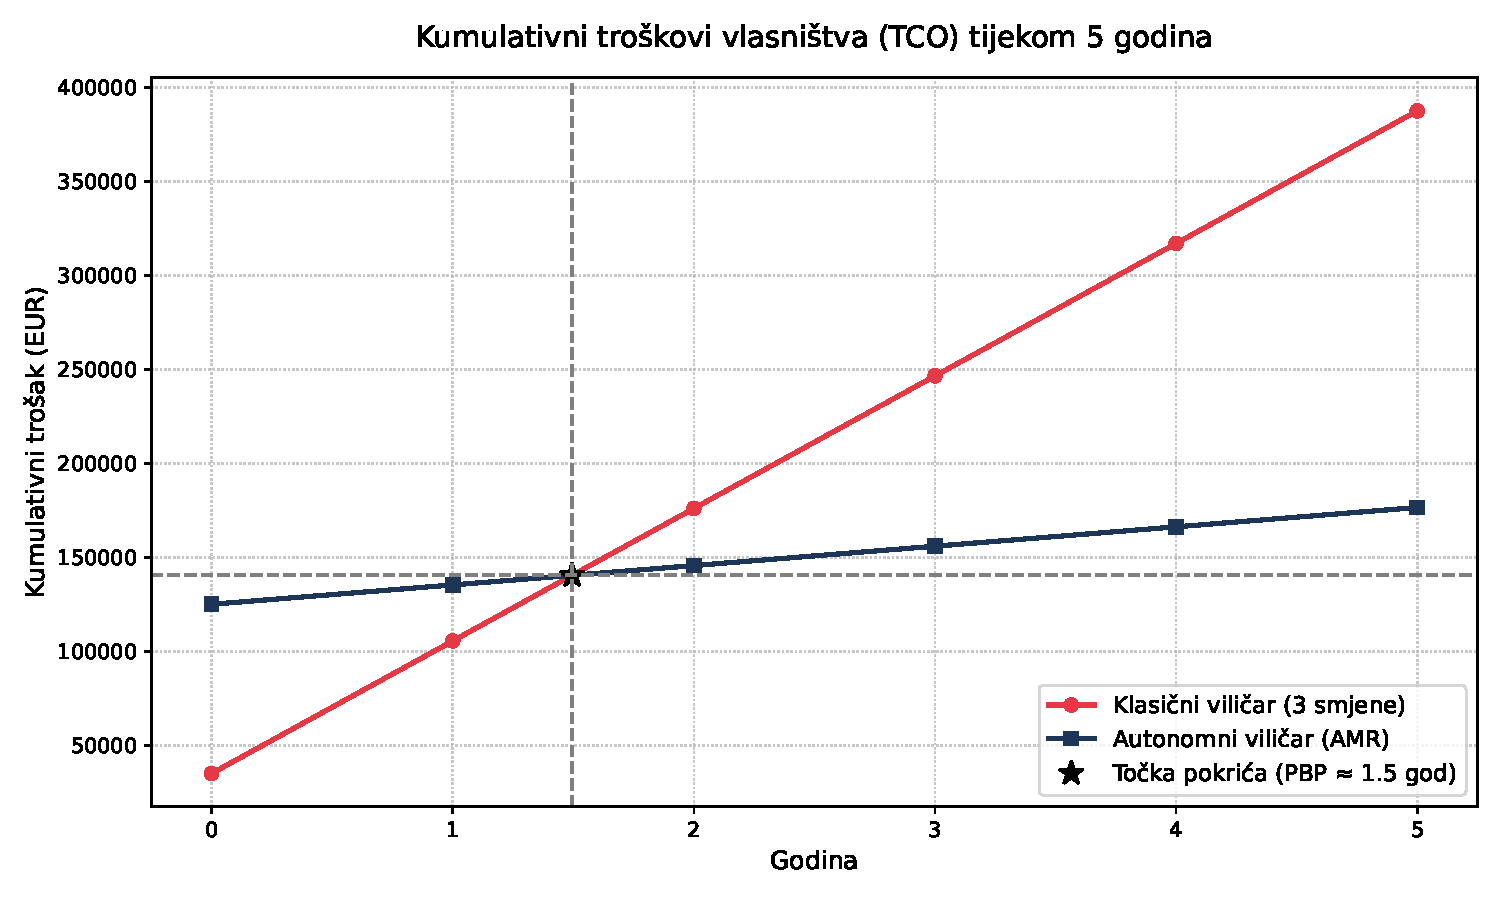
\includegraphics[width=0.9\textwidth]{slike/roi_chart.pdf}
\caption{Kumulativni troškovi vlasništva (TCO) tijekom 5 godina.}
\label{fig:roi_chart}
\end{figure}

Ekonomska analiza jasno pokazuje da je uvođenje autonomnih viličara izrazito opravdano u radnim okruženjima s visokim intenzitetom rada (2 ili više smjena) i visokim udjelom troškova ljudskog rada.

\subsection{Tehničko-tehnološka ograničenja i operativni izazovi}
Unatoč napretku tehnologije, autonomni viličari nisu univerzalno rješenje za sve probleme i zahtijevaju specifične radne uvjete:
\begin{enumerate}
    \item \textbf{Problem Wi-Fi/5G roaminga:} Stalna komunikacija s fleet managerom (npr. T-ONE) preduvjet je za rad. Prilikom kretanja kroz hodnike, viličar mora brzo i bez gubitka paketa prelaziti s jedne Wi-Fi pristupne točke (AP) na drugu. Ako prebacivanje traje dulje od 200 ms, sustav iz sigurnosnih razloga inicira zaustavljanje vozila. Rješavanje ovog problema zahtijeva značajne investicije u robusnu industrijsku mrežnu infrastrukturu.
    \item \textbf{Kvaliteta skladišnih podova (DIN 18202):} Prirodna navigacija i fuzija senzora uvelike se oslanjaju na odometriju. Ako su podovi neravni, imaju pukotine ili nagibe koji odstupaju od standarda DIN 18202, kotači viličara proklizavaju. To dovodi do akumulacije pogreške u Kalmanovom filtru i gubitka lokalizacije, kao i do opasnih vibracija tereta na velikim visinama.
    \item \textbf{Utjecaj okolišnih uvjeta:} Optoelektronički senzori (LiDAR-i i kamere) osjetljivi su na prašinu, vlagu i ekstremne promjene osvjetljenja. U skladištima s visokom koncentracijom suspendiranih čestica (papirna, drvna ili cementna industrija), senzori se moraju učestalo čistiti kako ne bi došlo do lažnih detekcija prepreka i zastoja u radu.
    \item \textbf{Nedostatak kognitivne fleksibilnosti:} Autonomni sustavi slijede stroge algoritamske obrasce. Ako viličar naiđe na stršeći komad plastične folije s palete, on će to prepoznati kao čvrstu prepreku i zaustaviti se, dok bi ljudski vozač procijenio da je prolazak siguran i nastavio vožnju.
\end{enumerate}

\clearpage
\section{ZAKLJUČAK}
Autonomni viličari i industrijska vozila predstavljaju ključni stup tranzicije prema konceptu pametnih skladišta i šire vizije *Industrije 4.0 \cite{kion}*. Tehnologija je prešla dug put od Barrettovog prvog žicom vođenog tegljača iz 1953. godine do današnjih visokosofisticiranih autonomnih viličara koji koriste SLAM algoritme, 3D LiDAR-e i računalni vid.

Glavni pokretač ove tranzicije je potreba za fleksibilnošću. Prirodna navigacija omogućila je uvođenje automatizacije u već postojeća skladišta bez potrebe za skupim građevinskim zahvatima i postavljenjem fizičkih vodiča. Sustavi fuzije senzora uspješno spajaju podatke s LiDAR-a, IMU-a, odometrije i kamera kako bi osigurali milimetarsku preciznost manipulacije teretom te maksimalnu sigurnost pješaka u skladu sa standardom ISO 3691-4.

Iako visoki inicijalni troškovi implementacije i održavanja te osjetljivost na vanjske uvjete predstavljaju izazove za mala i srednja poduzeća, prednosti u vidu 24-satnog rada, dramatičnog smanjenja oštećenja robe i optimizacije procesa čine ovu tehnologiju ekonomski isplativom na srednji i dugi rok. Budući razvoj intralogistike bit će obilježen daljnjom integracijom umjetne inteligencije za prediktivnu analizu tokova materijala, uvođenjem 5G mreža za bržu komunikaciju flote te razvojem hibridnih kolaborativnih sustava u kojima ljudi i autonomni strojevi rade u sinergiji.

\clearpage

\printbibliography[heading=bibintoc, title={LITERATURA}]

\end{document}
